\documentclass[../proyecto.tex]{memoir}

\begin{document}

\chapter{Análisis}

%\section{$\alpha$-asincronismo en la evolución de las configuraciones iniciales}

En esta sección vamos a estudiar el impacto de la $\alpha$-asíncronicidad sobre las configuraciones iniciales escogidas en la sección \ref{seleccion}. Las ejecuciones son de 50 iteraciones, cada iteración simulada 5000 veces, con los valores de $\alpha$: 0.15, 0.3, 0.45, 0.6, 0.75 y 0.9. En las gráficas de múltiples valores de $\alpha$ se muestra también el valor $\alpha=1$ para poder comparar el comportamiento $\alpha$-asíncrono con el síncrono. Como resultado hemos obtenido los valores medios de las variables expuestas en la sección \ref{vars} junto con sus correspondientes intervalos de confianza para cada iteración.

\subsection{Hipótesis de normalidad} \label{normalidad}

Para que las estimaciones Monte Carlo tengan los intervalos de confianza tengan el significado que se les da en la sección \ref{carlino}, es necesario comprobar que la distribución del estimador de la media sigue una distribución normal. Para ello aplicamos el de test de normalidad de Shapiro-Wilk\cite{shapiro} con un nivel de significancia de 0.05. En nuestra sitación la hipótesis nula, $H_0$, es que el estimador de la media sigue una distribución normal y la hipótesis alternativa $H_1$ es que sigue una distribución distinta a la normal. Con este test no podremos afirmar que definitivamente la distribución sea normal por lo que nos reduciremos a afirmar que no podemos negar que la distribución sea normal, esto es, no rechazar la hipótesis nula. Una buena propiedad de este test, la cual ha motivado su elección, es que la probabilidad de rechazar la hipótesis nula cuando es cierta es aproximadamente del 5\% independientemente del tamaño de la muestra \cite{powertest}.

En la \autoref{fig:alpha} es posible observar como para cada iteración tenemos representado el intervalo de confianza $[\mu-3*\sigma, \mu+3*\sigma]$, junto con el punto central del intervalo: $\mu$, la media del estimador. En las situaciones en las cuales el $p-value$ generado por el test de normalidad no supera el nivel de significación se ha pintado de color naranja, es decir, las situaciones en las que se rechaza $H_0$ y en otro caso de color azul. En caso de que la hipótesis nula sea rechazada tan solo podemos afirmar que la media del estimador converge en probabilidad como se comenta en la sección \ref{carlino}.

\begin{figure}[H]
	\centering
    \includegraphics[width=0.9\textwidth]{./images/data/lightweightspaceship/{iteracion_Area_0.30_5000_50}.png}
    \caption{Promedio de densidad para $\alpha$=0.3 de la configuración \textit{lightweight spaceship}.}
    \label{fig:alpha}
\end{figure}

Notar que para valores extremos de $\alpha$ hemos observado que se pueden encontrar situaciones en la cuales se rechace más a menudo la hipótesis de normalidad, como las que se muestran en la \autoref{fig:tiste}. Entendemos que esta situación se da porque si existe un número de simulaciones a partir del cual el estimador sigue una distribución normal, aún no se ha alcanzado. Otra situación posible en la que se rechace la hipótesis de normalidad para casi todas las iteraciones es que los valores obtenidos sean constantes en todas las simulaciones y por tanto el estimador converge en probabilidad trivialmente como se muestra en la \autoref{fig:alpha2} pero sin seguir una distribución normal.

\begin{figure}[H]
	\centering
    \includegraphics[width=0.8\textwidth]{./images/data/glider/{iteracion_Celulas_0.99_5000_50}.png}
    \caption{Promedio de nodos ocupados para $\alpha$=0.99 de la configuración \textit{glider}.}
    \label{fig:tiste}
\end{figure}


\begin{figure}[H]
	\centering
    \includegraphics[width=0.9\textwidth]{./images/data/lightweightspaceship/{iteracion_Clusteres_0.99_5000_50}.png}
    \caption{Promedio de clústeres para $\alpha$=0.99 de la configuración \textit{lightweight spaceship}.}
    \label{fig:alpha2}
\end{figure}

\subsection{\textit{Osciladores} de periodo 2} \label{osci2}

Comenzamos el análisis con la \autoref{fig:blinker_evo}. Cuando no existe perturbación en el intercambio de información entre nodos ocupados, el calor en cada iteración es de 4 \textit{nodos}, ocupa un área de 3 \textit{nodos}$^2$ y está conformada por un solo clúster de 3 nodos ocupados. En primer lugar destacamos que independientemente al valor que tome $\alpha$ el número medio de clústeres es constantemente la unidad.

Si observamos la \autoref{fig:blinker_calor} es posible ver que los valores medios permanecen aproximadamente constantes para cada valor de $\alpha$. Además a medida que $\alpha$ se aproxima a la unidad, el promedio de calor se aproxima al que se obtiene en condiciones síncronas de evolución. También que puede observar notablemente que la variación de $\alpha$ produce que el calor medio varíe en más de 3 unidades, lo que nos hace pensar que el efecto de la $\alpha$-asincronicidad sobre esta configuración ralentiza la evolución de la misma. En la \autoref{fig:blinker_alpha_calor} se observa con más claridad la evolución del calor medio junto con su desviación estándar frente al valor de $\alpha$

Notar que el hecho de que los valores medios permanecen constantes independientemente al valor que tome $\alpha$ se da en todas las configuraciones, por lo que de ahora en adelante lo omitiremos.

Por otro lado, en la \autoref{fig:blinker_alpha_area} se observa un comportamiento distinto al anterior. Se mantiene el hecho de que para valores de $\alpha$ cercanos a la unidad, el promedio se aproxima de forma continua al que se da bajo situación de sincronicidad. En el rango de valores de $\alpha\in[0.15,\ 0.6]$ se observa que el área media crece hasta alcanzar su máximo valor cercano a 4 \textit{nodos}$^2$ cuando $\alpha$ crece hasta 0.45, sin embargo a partir de este valor de $\alpha$ los promedios descienden hasta 3.5 \textit{nodos}$^2$ en $\alpha=0.75$. %Este comportamiento descrito para el área media es muy similar al que se da para el número medio de vidas inmóviles.

\begin{figure}[H]
	\centering
    \includegraphics[width=0.8\textwidth]{./images/data/blinker/{Calor_multiple_alpha}.png}
    \caption{Evolución $\alpha$-asíncrona del calor medio de la configuración \textit{blinker}.}
    \label{fig:blinker_calor}
\end{figure}

\begin{figure}[H]
	\centering
    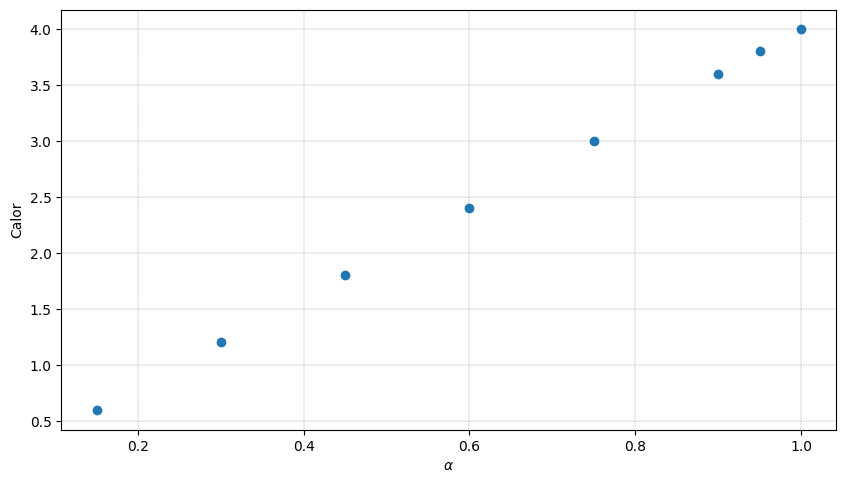
\includegraphics[width=\textwidth]{./images/data/blinker/alpha_Calor.png}
    \caption{Evolución $\alpha$-asíncrona del calor medio de la configuración \textit{blinker}.}
    \label{fig:blinker_alpha_calor}
\end{figure}

\begin{figure}[H]
	\centering
    \includegraphics[width=\textwidth]{./images/data/blinker/{alpha_Area}.png}
    \caption{Evolución $\alpha$-asíncrona del área media de la configuración \textit{blinker}.}
    \label{fig:blinker_alpha_area}
\end{figure}

Tanto la densidad media como el promedio de vidas inmóviles y el promedio de células varían sutilmente, es decir, la longitud del intervalo en el que suceden los cambios es a lo sumo de 0.5 unidades, por tanto omitimos su análisis.

El otro oscilador de periodo dos que hemos estudiado, \textit{toad}, (\autoref{fig:toad_evo}) está formado por 6 nodos ocupados que ocupan un área de 8 \textit{nodos}$^2$ en las iteraciones pares y 16 \textit{nodos}$^2$ en las impares. A diferencia de la configuración anterior tanto el área como el calor medios experimentan un comportamiento muy similar en situación de $\alpha$-asíncronicidad al descrito en la \autoref{fig:blinker_calor}. 

El número de clústeres medio deja de ser constante y varía en aproximadamente una unidad para los distintos valores de $\alpha$ (\autoref{fig:toad_alpha_clusters} y \autoref{fig:toad_clusters}). Por último la densidad media de esta configuración varía sutilmente y omitimos su análisis.

\begin{figure}[H]
	\centering
    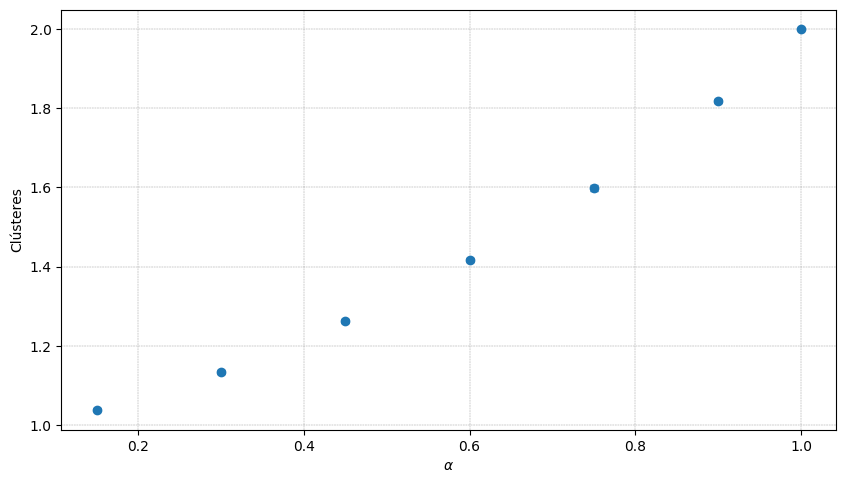
\includegraphics[width=\textwidth]{./images/data/toad/alpha_Clusteres.png}
    \caption{Evolución $\alpha$-asíncrona del número de clústeres medio de la configuración \textit{toad}.}
    \label{fig:toad_alpha_clusters}
\end{figure}


\begin{figure}[H]
		\centering
    	\includegraphics[width=0.8\textwidth]{./images/data/toad/{Clusteres_multiple_alpha}.png}
    \caption{Evolución $\alpha$-asíncrona del número de clústeres medio de la configuración \textit{toad}.}
    \label{fig:toad_clusters}
\end{figure}


\subsection{\textit{Osciladores} de periodo 3}

En la \autoref{fig:jam_evo} podemos observar tres iteraciones de la configuración \textit{jam}, la cual curiosamente contiene una vida inmóvil. En situación de actualización síncrona esta configuración inicial está formada por 13 nodos ocupados agrupados en tres clústeres y ocupa un área de 42 \textit{nodos}$^2$. En su primera iteración se incrementa el número de nodos a 16, agrupados en un clúster y con un calor de 4 nodos, manteniendo el mismo área. La siguiente iteración incrementa su área a 49 \textit{nodos}$^2$, disminuyendo el número de nodos ocupados a 14, agrupados en dos clústeres con un calor de 9 nodos. Al avanzar una iteración más, la configuración retorna al estado de la configuración inicial. 

\begin{figure}[H]
	\centering
    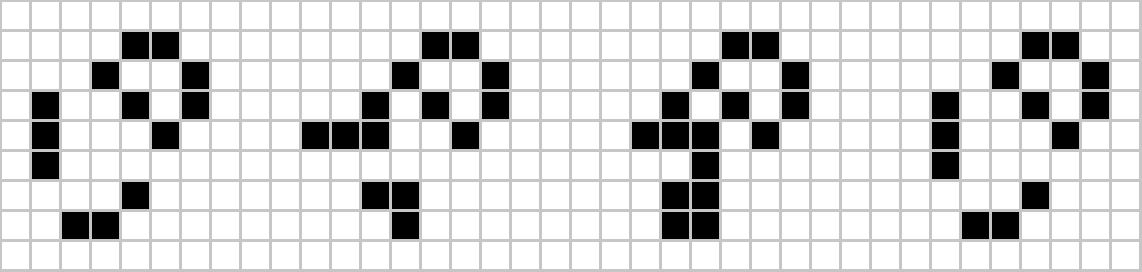
\includegraphics[width=0.9\textwidth]{./images/jam_evo.png}
    \caption{De izquierda a derecha, evolución síncrona de la configuración \textit{jam}.}
    \label{fig:jam_evo}
\end{figure}

En esta configuración se observa el mismo comportamiento para los promedios de área y calor que para la configuración \textit{toad}. Por el contrario, para el número medio de clústeres (\autoref{fig:jam_alpha_clusters} y \autoref{fig:jam_clusters}) se tiene el comportamiento opuesto, esto es, el valor decrece con el crecimiento de $\alpha$, siendo su máximo valor cercano a 2.7 clústeres para $\alpha=0.15$ y su mínimo próximo 2 clústeres para $\alpha=0.9$.

\begin{figure}[H]
	\centering
    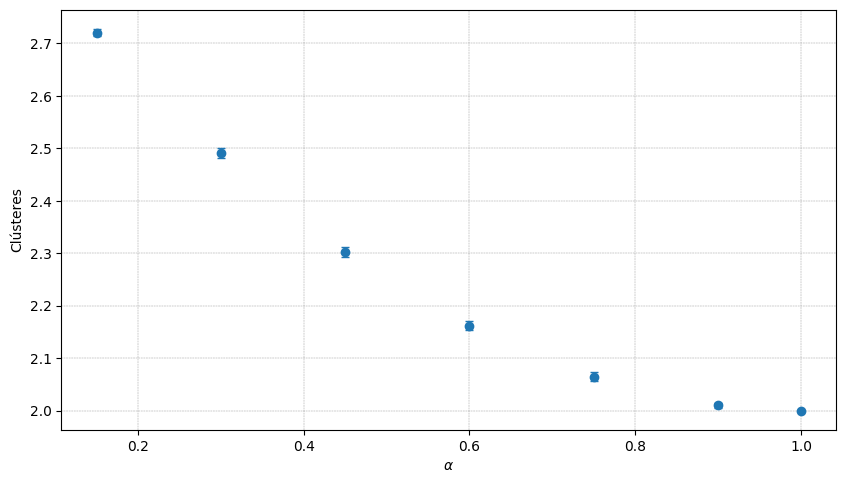
\includegraphics[width=\textwidth]{./images/data/jam/alpha_Clusteres.png}
    \caption{Evolución $\alpha$-asíncrona del promedio de clústeres de la configuración \textit{jam}.}
    \label{fig:jam_alpha_clusters}
\end{figure}

\begin{figure}[H]
		\centering
    	\includegraphics[width=0.8\textwidth]{./images/data/jam/{Clusteres_multiple_alpha}.png}
    \caption{Evolución $\alpha$-asíncrona del promedio de clústeres de la configuración \textit{jam}.}
    \label{fig:jam_clusters}
\end{figure}

A continuación, en la \autoref{fig:pulsar_evo} podemos observar tres iteraciones de la configuración \textit{pulsar}, la cual es notablemente la configuración de mayor tamaño que hemos estudiado. En situación de actualización síncrona esta configuración inicial está formada por 48 nodos ocupados agrupados en 12 clústeres y ocupa un área de 169 \textit{nodos}$^2$. En su primera iteración se incrementa el número de nodos a 72, agrupados en el mismo número de clústeres y con un calor de 32 nodos, incrementando el área a 225\textit{nodos}$^2$. La siguiente iteración retorna su área a 169 \textit{nodos}$^2$, manteniendo el número de nodos ocupados, agrupados en 4 clústeres con un calor de 40 nodos. Al avanzar una iteración más, la configuración retorna al estado de la configuración inicial con un calor de 56 nodos. 

\begin{figure}[H]
	\centering
    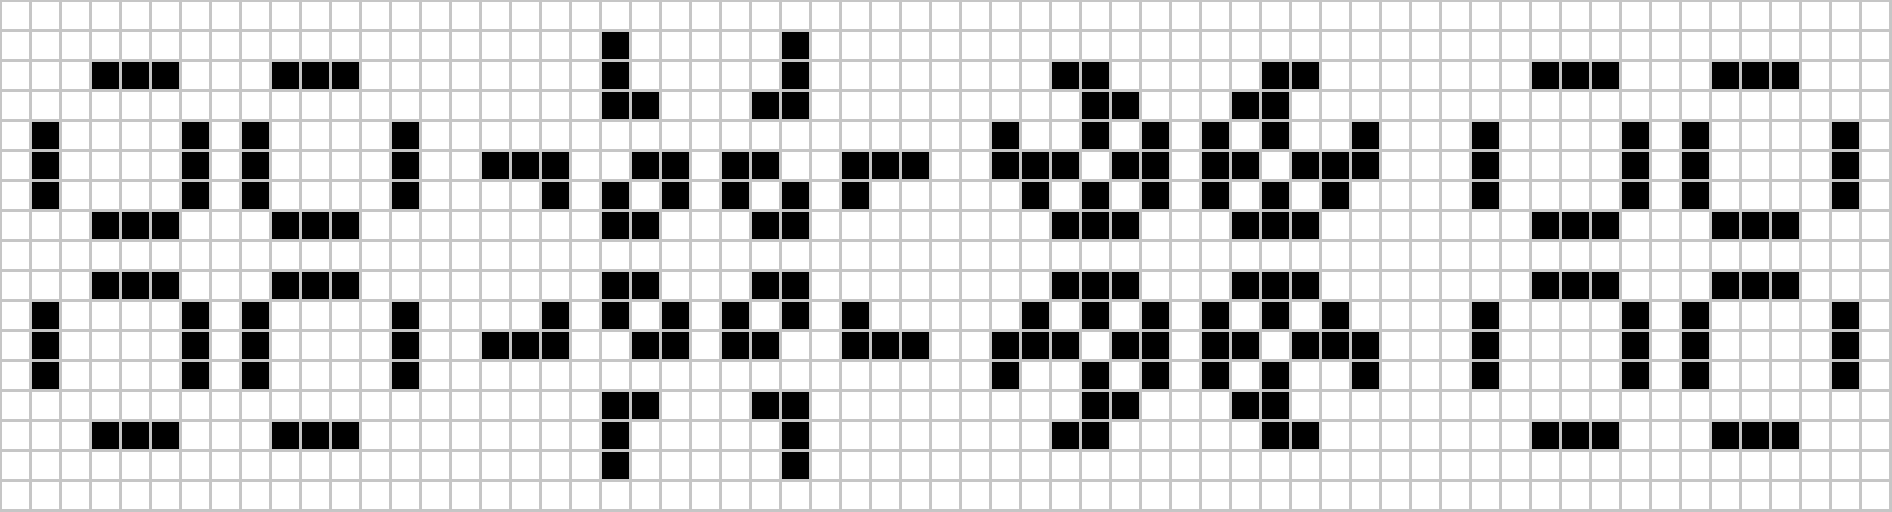
\includegraphics[width=\textwidth]{./images/pulsar_evo.png}
    \caption{De izquierda a derecha, evolución síncrona de la configuración \textit{pulsar}.}
    \label{fig:pulsar_evo}
\end{figure}

Esta configuración experimenta el mismo comportamiento en el calor medio que la configuración \textit{jam}. Por otra parte la variación del área media (\autoref{fig:pulsar_area}) es similar, notando que la separación entre los valores medios crece respecto de $\alpha$, alcanzando para $\alpha=0.9$ un valor medio próximo a los 225 \textit{nodos}$^2$ de la primera iteración síncrona de esta configuración. 

El número medio de clústeres (\autoref{fig:pulsar_clusteres} y \autoref{fig:pulsar_alpha_clusteres}) decrece de $\alpha=0.15$ a $\alpha=0.6$ una unidad, a continuación crece 1.25 clústeres de $\alpha=0.6$ a $\alpha=0.9$. Además en la (\autoref{fig:pulsar_fijas} y \autoref{fig:pulsar_alpha_fijas}) el número de vidas inmóviles crece casi 1.5 unidades respecto de $\alpha$.


\begin{figure}[H]
		\centering
    	\includegraphics[width=0.75\textwidth]{./images/data/pulsar/{Area_multiple_alpha}.png}
    \caption{Evolución $\alpha$-asíncrona del promedio de área de la configuración \textit{pulsar}.}
    \label{fig:pulsar_area}
\end{figure}


\begin{figure}[H]
		\centering
    	\includegraphics[width=0.75\textwidth]{./images/data/pulsar/{Clusteres_multiple_alpha}.png}
    \caption{Evolución $\alpha$-asíncrona del promedio de clústeres de la configuración \textit{pulsar}.}
    \label{fig:pulsar_clusteres}
\end{figure}

\begin{figure}[H]
	\centering
    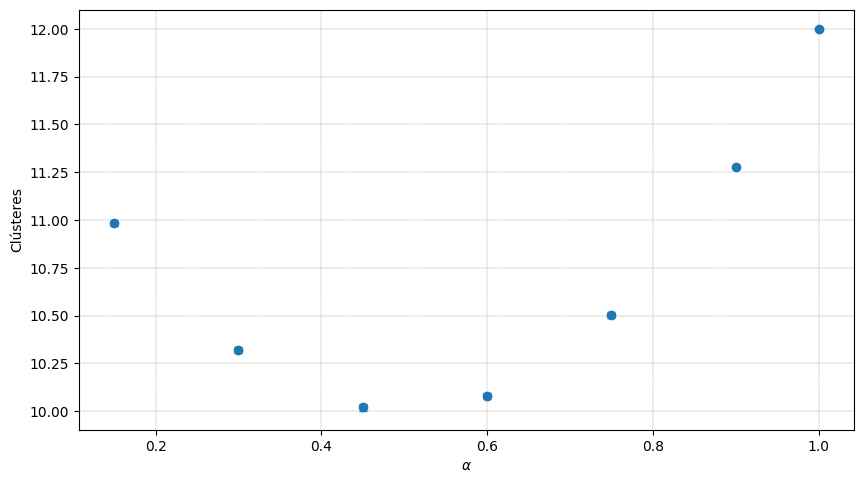
\includegraphics[width=\textwidth]{./images/data/pulsar/alpha_Clusteres.png}
    \caption{Evolución $\alpha$-asíncrona del promedio de clústeres de la configuración \textit{pulsar}.}
    \label{fig:pulsar_alpha_clusteres}
\end{figure}

\begin{figure}[H]
		\centering
    	\includegraphics[width=0.8\textwidth]{./images/data/pulsar/{Fijas_multiple_alpha}.png}
    \caption{Evolución $\alpha$-asíncrona del promedio de vidas inmóviles de la configuración \textit{pulsar}.}
    \label{fig:pulsar_fijas}
\end{figure}

\begin{figure}[H]
	\centering
    \includegraphics[width=\textwidth]{./images/data/pulsar/{alpha_Fijas}.png}
    \caption{Evolución $\alpha$-asíncrona del promedio de vidas inmóviles de la configuración \textit{pulsar}.}
    \label{fig:pulsar_alpha_fijas}
\end{figure}

\subsection{\textit{Osciladores} de periodo 4}

En esta sección estudiaremos la variación $\alpha$-asíncrona de las configuraciones \textit{mold} y \textit{mazing}. En la \autoref{fig:mold_evo} es posible observar la 4 iteraciones de la evolución en condiciones de sincronicidad de la configuración \textit{mold}. Esta configuración inicial cuenta con 12 nodos ocupados, agrupados en dos clústeres con un área de 36 \textit{nodos}$^2$. En su primera iteración genera un calor de 8 nodos, variando tanto el número de nodos ocupados como el área que ocupan, a 14 nodos ocupados y 30 \textit{nodos}$^2$, agrupados en un solo cluster. Esta iteración genera un calor de 6 nodos. La siguiente iteración la configuración retorna al mismo área, nodos ocupados y clústeres de la configuración inicial pero en diferente disposición, con un calor de 8. La tercera iteración ocupa un área de 30 \textit{nodos}$^2$, que se reparten 14 nodos ocupados en un único clúster con un calor de 6. En la cuarta iteración la configuración coincide con la configuración inicial con un calor de 8 nodos.

\begin{figure}[H]
	\centering
    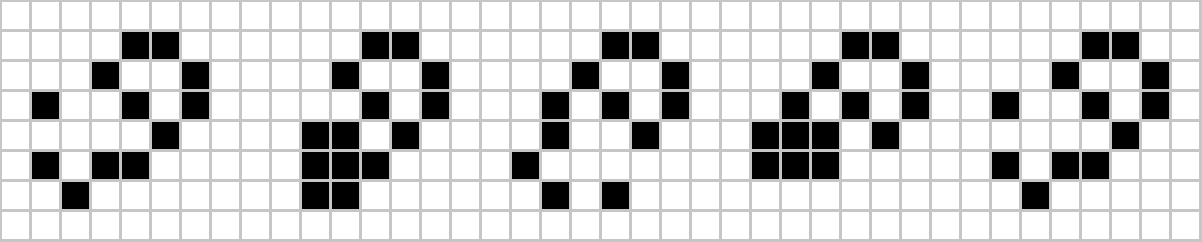
\includegraphics[width=\textwidth]{./images/mold_evo.png}
    \caption{De izquierda a derecha, evolución síncrona de la configuración \textit{mold}.}
    \label{fig:mold_evo}
\end{figure}

Esta configuración tiene en común con la configuración \textit{blinker} que el promedio de clústeres permanece constante en la unidad. Además el calor medio se comporta de la misma manera que en la configuración \textit{blinker}, solo que en lugar de crecer aproximadamente 0.5 nodos, crece 0.75 nodos respecto de $\alpha$.

El área media varía de una forma muy curiosa (\autoref{fig:mold_area}). En lugar de crecer con el valor de $\alpha$, decrece obteniendo el mayor valor, 36 \textit{nodos}$^2$, para $\alpha=0.15$ y el menor, 30.5 \textit{nodos}$^2$, para $\alpha=0.9$. Además el crecimiento respecto de $\alpha$ es constante, aproximadamente una unidad. Análogamente, el número medio de nodos ocupados crece respecto de $\alpha$ aproximadamente una unidad, alcanzando su máximo, 14 nodos ocupados, para $\alpha=0.15$ y su mínimo, 11.5 nodos ocupados, para $\alpha=0.9$ (\autoref{fig:mold_celulas}).

\begin{figure}[H]
		\centering
    	\includegraphics[width=0.8\textwidth]{./images/data/mold/{Area_multiple_alpha}.png}
    \caption{Evolución $\alpha$-asíncrona del área media de la configuración \textit{mold}.}
    \label{fig:mold_area}
\end{figure}

\begin{figure}[H]
		\centering
    	\includegraphics[width=0.8\textwidth]{./images/data/mold/{Celulas_multiple_alpha}.png}
    \caption{Evolución $\alpha$-asíncrona del promedio de nodos ocupados de la configuración \textit{mold}.}
    \label{fig:mold_celulas}
\end{figure}


En la \autoref{fig:mazing_evo} es posible observar la 4 iteraciones de la evolución en condiciones de sincronicidad de la configuración \textit{mazing}. Esta configuración inicial cuenta con 12 nodos ocupados, agrupados en 4 clústeres con un área de 49 \textit{nodos}$^2$. En su primera iteración genera un calor de 14 nodos, variando tanto el número de nodos ocupados como el de clústeres a 18 nodos ocupados y un clúster, manteniendo el área anterior. Esta iteración genera un calor de 14 nodos. La siguiente iteración la configuración retorna al mismo área, nodos ocupados y clústeres de la configuración inicial pero en diferente disposición, con un calor de 14 nodos. La tercera iteración tiene el mismo área, nodos ocupados y clústeres de la primera iteración pero en diferente disposición con un calor de 14 nodos. En la cuarta iteración la configuración coincide con la configuración inicial.

\begin{figure}[H]
	\centering
    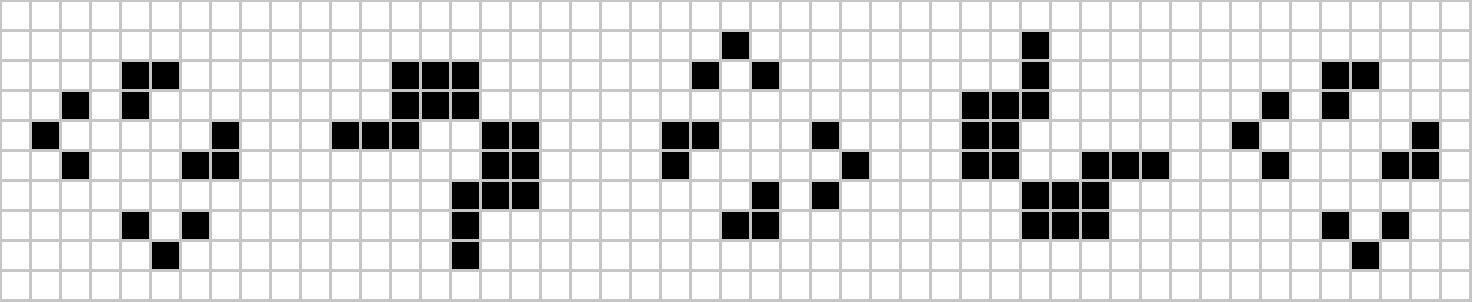
\includegraphics[width=\textwidth]{./images/mazing_evo.png}
    \caption{De izquierda a derecha, evolución síncrona de la configuración \textit{mazing}.}
    \label{fig:mazing_evo}
\end{figure}

En esta configuración destaca el hecho de que el área permanezca constante en 49 \textit{nodos}$^2$ independientemente al valor de $\alpha$. Por otra parte tanto el calor medio como el número de nodos ocupados tienen el mismo comportamiento, crecen respecto de $\alpha$, la única diferencia es que en el primero el incremento respecto de $\alpha$ es de dos unidades y en el segundo de tan solo una unidad. Dicho comportamiento es común a la configuración anterior, \textit{mold}.

El promedio de vidas inmóviles decrece respecto de $\alpha$ pero no lo hace en la misma medida que el calor medio, si no que para los valores de $\alpha\leq 0.6$ es prácticamente el mismo decrecimiento, siendo el valor máximo $\alpha=0.15$ con algo más de 1.5 vidas inmóviles en media (\autoref{fig:mazing_fijas} y \autoref{fig:mazing_alpha_fijas}). Sin embargo a partir de este valor, el incremento disminuye rápidamente y el promedio de vidas inmóviles se aproxima a 0.

\begin{figure}[H]
		\centering
    	\includegraphics[width=\textwidth]{./images/data/mazing/{alpha_Fijas}.png}
    \caption{Evolución $\alpha$-asíncrona del promedio de vidas inmóviles de la configuración \textit{mazing}.}
    \label{fig:mazing_alpha_fijas}
\end{figure}

\begin{figure}[H]
		\centering
    	\includegraphics[width=0.8\textwidth]{./images/data/mazing/{Fijas_multiple_alpha}.png}
    \caption{Evolución $\alpha$-asíncrona del promedio de vidas inmóviles de la configuración \textit{mazing}.}
    \label{fig:mazing_fijas}
\end{figure}

Por último, el número medio de clústeres decrece respecto de $\alpha$ (\autoref{fig:mazing_clusteres}) pero de nuevo no es en la misma medida que el calor medio, si no que de $\alpha=0.15$ a $\alpha=0.3$ y de $\alpha=0.75$ a $\alpha=0.9$ el incremento es aproximadamente el mismo, 0.5 clústeres y los decrementos para los valores restantes de $\alpha$ son aproximadamente 0.25 clústeres.

\begin{figure}[H]
		\centering
    	\includegraphics[width=0.8\textwidth]{./images/data/mazing/{Clusteres_multiple_alpha}.png}
    \caption{Evolución $\alpha$-asíncrona del promedio de clústeres de la configuración \textit{mazing}.}
    \label{fig:mazing_clusteres}
\end{figure}

\subsection{\textit{Naves espaciales}}
Hasta ahora solo hemos descrito el comportamiento de \textit{osciladores}. Como se expuso en la sección \ref{spaceships}, las \textit{naves espaciales} pueden ser vistas como \textit{osciladores} que se desplazan, luego es interesante explorar si los comportamientos que hemos observado en las configuraciones iniciales anteriores se reproducen en este tipo de configuraciones iniciales. 

Comenzamos la sección estudiando la configuración inicial \textit{lightweight spaceship} (\autoref{fig:lightweightspaceship}). En la \autoref{fig:lightweightspaceship_evo} se muestran 4 iteraciones de esta configuración inicial. Se trata de una configuración de velocidad $c/2$ que se desplaza paralelamente al eje horizontal con un área constante de 20 \textit{nodos}$^2$. En las iteraciones pares tiene 9 nodos ocupados agrupados en dos clústeres con un calor de 9 nodos y en las iteraciones impares tiene 12 nodos agrupados en un solo clúster con un calor de 13 nodos.

\begin{figure}[H]
	\centering
    
\includegraphics[width=\textwidth]{./images/lightweightspaceship_evo.png}
    \caption{De derecha a izquierda, evolución síncrona de la configuración \textit{lightweight spaceship}.}
    \label{fig:lightweightspaceship_evo}
\end{figure}

Uno de los característicos efectos que produce la introducción de $\alpha$-asincronismo en esta configuración inicial es que el número medio de clústeres permanece constante en todas las ejecuciones como en la configuración \textit{blinker}. Además el número de vidas inmóviles es constantemente 0 independientemente al valor de $\alpha$. Si observamos el número medio de nodos ocupados (\autoref{fig:7-2}) se observa que la separación vertical de los valores medios constantes es aproximadamente igual a 0.5 nodos ocupados entre valores consecutivos de $\alpha$. De esta manera el observamos que cuando el valor de $\alpha$ el promedio nodos ocupados se acerca a los 12 nodos ocupados en la iteraciones impares de esta configuración con la evolución síncrona.

Mientras que la densidad y el calor medios de esta configuración tienen un comportamiento similar al número medio de nodos ocupados se puede observar una variación diferente en el área media (\autoref{fig:7-3} y \autoref{fig:7-4}). Cuando $\alpha$ se aproxima, tanto inferior como superiormente, a $0.5$ los valores medios de área se estabilizan entorno al valor 21.2 \textit{nodos}$^2$. Por otro lado cuando $\alpha$ se aproxima a 0 ó a 1, los valores medios se aproximan a 20.5 \textit{nodos}$^2$, un valor muy cercano a los 20 \textit{nodos}$^2$ de la configuración con evolución síncrona. Otra cuestión notable es que el valor de área media varía en el intervalo de una unidad de longitud cuando $\alpha$ varía. A diferencia de la longitud de los intervalos en los que se encuentran los promedios de nodos ocupados, densidad y calor, que es mayor.

\begin{figure}[H] 
    \centering
    \includegraphics[width=0.76\textwidth]{./images/data/lightweightspaceship/{Celulas_multiple_alpha}.png}
    \caption{Evolución $\alpha$-asíncrona del promedio de nodos ocupados de la configuración \textit{lightweight spaceship}.}
    \label{fig:7-2}
\end{figure}
 
\begin{figure}[H]
	\centering
    \includegraphics[width=0.76\textwidth]{./images/data/lightweightspaceship/{Area_multiple_alpha}.png}
    \caption{Evolución $\alpha$-asíncrona del área media de la configuración \textit{lightweight spaceship}.}
    \label{fig:7-3}
\end{figure}

\begin{figure}[H]
	\centering
    \includegraphics[width=\textwidth]{./images/data/lightweightspaceship/{alpha_Area}.png}
    \caption{Evolución $\alpha$-asíncrona del área media de la configuración \textit{lightweight spaceship}.}
    \label{fig:7-4}
\end{figure}

La configuración inicial \textit{middleweight spaceship} (\autoref{fig:middleweightspaceship}) tiene un aspecto y una evolución síncrona similar a la configuración \textit{lightweight spaceship}. En la \autoref{fig:middleweightspaceship_evo} se muestran 4 iteraciones de esta configuración inicial. Se trata de una configuración de velocidad $c/2$ que se desplaza paralelamente al eje horizontal con un área constante de 24 \textit{nodos}$^2$. En las iteraciones pares tiene 11 nodos ocupados agrupados en tres clústeres con un calor de 12 nodos y en las iteraciones impares tiene 15 nodos agrupados en un solo clúster con un calor de 18 nodos.

\begin{figure}[H]
	\centering
    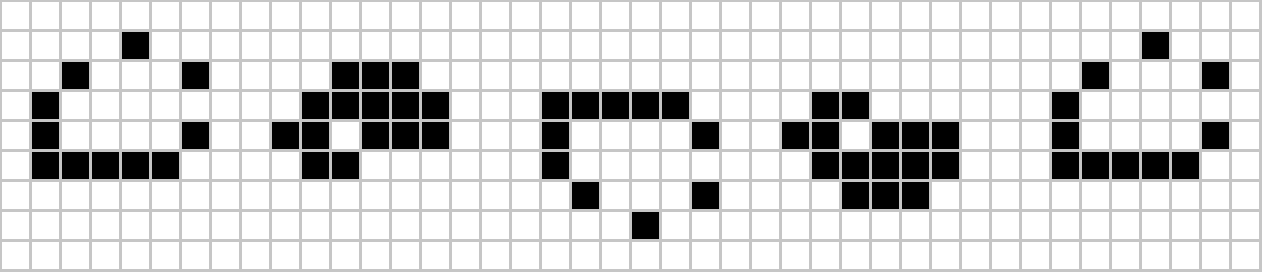
\includegraphics[width=\textwidth]{./images/middleweightspaceship_evo.png}
    \caption{De derecha a izquierda, evolución síncrona de la configuración \textit{middleweight spaceship}.}
    \label{fig:middleweightspaceship_evo}
\end{figure}

Al igual que en la configuración anterior, \textit{lightweight spaceship}, el número de clústeres y el de vidas inmóviles permanece constante independientemente del valor de $\alpha$. Y tanto el promedio de nodos ocupados como el de densidad tienen el mismo comportamiento. Sin embargo para el valor medio de área se produce una variación del comportamiento que se puede observar en la \autoref{fig:88-1} y en la \autoref{fig:88}. El área varía prácticamente de la misma manera para $\alpha=0.15,\ 0.75$ y a excepción de $\alpha=0.90$ el resto de valores de $\alpha$ muestran un comportamiento constante muy parecido entre sí. 

\begin{figure}[H]
	\centering
    \includegraphics[width=\textwidth]{./images/data/middleweightspaceship/{alpha_Area}.png}
    \caption{Evolución $\alpha$-asíncrona del área media de la configuración \textit{middleweight spaceship}.}
    \label{fig:88-1}
\end{figure}


\begin{figure}[H]
	\centering
    \includegraphics[width=0.8\textwidth]{./images/data/middleweightspaceship/{Area_multiple_alpha}.png}
    \caption{Evolución $\alpha$-asíncrona del área media de la configuración \textit{middleweight spaceship}.}
    \label{fig:88}
\end{figure}


Por otro lado, una diferencia notable con la configuración anterior es que la longitud del intervalo en el que varía el promedio crece aproximadamente una unidad más.

La siguiente configuración que vamos a estudiar, \textit{heavyweight spaceship} muestra un aspecto similar a las dos anteriores tanto en forma como en su evolución síncrona. En la \autoref{fig:heavyweightspaceship_evo} se muestran 4 iteraciones de esta configuración inicial. Se trata de una configuración de velocidad $c/2$ que se desplaza paralelamente al eje horizontal con un área constante de 35 \textit{nodos}$^2$. En las iteraciones pares tiene 13 nodos ocupados agrupados en tres clústeres con un calor de 15 nodos y en las iteraciones impares tiene 18 nodos agrupados en un solo clúster con un calor de 23 nodos.

\begin{figure}[H]
	\centering
    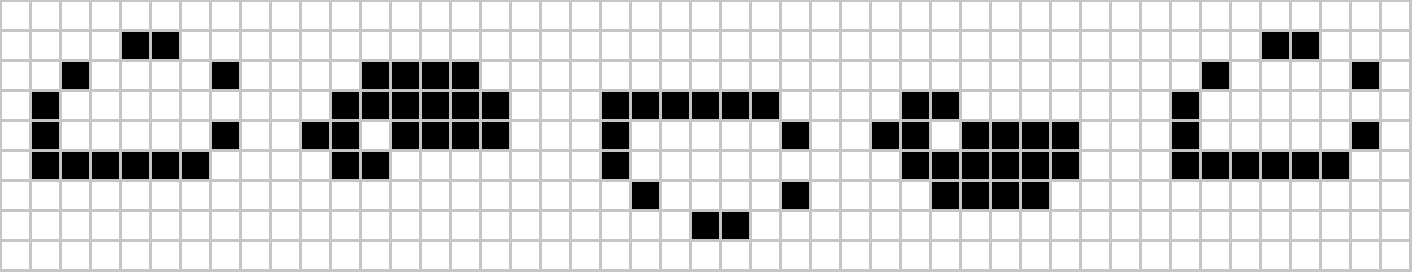
\includegraphics[width=\textwidth]{./images/heavyweightspaceship_evo.png}
    \caption{De derecha a izquierda, evolución síncrona de la configuración \textit{heavyweight spaceship}.}
    \label{fig:heavyweightspaceship_evo}
\end{figure}

A diferencia de las anteriores \textit{naves espaciales}, en la configuración \textit{heavyweight spaceship} el número de clústeres no se mantiene constante independientemente del valor que $\alpha$ tome. Aunque el número de vidas inmóviles si continúa siendo constantemente 0. En la \autoref{fig:9-1} es posible observar este cambio, además todos los valores medios se mantienen aproximadamente constantes a partir de la décima iteración. A medida que $\alpha$ incrementa se visualiza que la separación vertical de los valores del promedio de clústeres no es constante como en las \textit{naves espaciales} anteriores (\autoref{fig:7-2}) y dicha separación incrementa con el valor de $\alpha$.

Para el valor medio de área, el intervalo en el que oscila para distintos valores de $\alpha$ crece hasta una longitud de 8 \textit{nodos}$^{-1}$, siendo para $\alpha=0.9$ el menor valor de área, 31 \textit{nodos}$^2$ y para $\alpha=0.30, 0.45$ los mayores valores medios, aproximadamente 39 \textit{nodos}$^2$.

Los promedios de calor y número de nodos ocupados muestran un comportamiento idéntico al que se puede observar en la \autoref{fig:7-2}.

\begin{figure}[H]
	\centering
    \includegraphics[width=0.8\textwidth]{./images/data/heavyweightspaceship/{Clusteres_multiple_alpha}.png}
    \caption{Variación del promedio de clústeres en la configuración \textit{heavyweight spaceship} para distintos valores de $\alpha$.}
    \label{fig:9-1}
\end{figure}

Por último, la configuración inicial \textit{glider} es una nave espacial de velocidad $c/4$ formada por 5 nodos ocupados agrupados en un único clúster, tiene un calor de 4 \textit{nodos} y ocupa un área de 9 \textit{nodos}$^2$ (\autoref{fig:glider_evo}). De esta figura destacamos que el calor medio se desarrolla de forma similar al que hemos observado para la configuración \textit{blinker} al igual que lo hace el área media pero en intervalos de mayor longitud (\autoref{fig:9-4} y \autoref{fig:9-5}). Mientras que los promedios restantes varían sutilmente en intervalos de muy reducida longitud.

\begin{figure}[H]
	\centering
    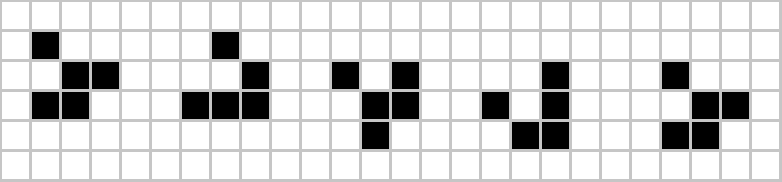
\includegraphics[width=0.7\textwidth]{./images/glider_evo.png}
    \caption{De izquierda a derecha, evolución síncrona de la configuración \textit{glider}.}
    \label{fig:glider_evo}
\end{figure}

\begin{figure}[H] 
    \centering
    \includegraphics[width=0.8\textwidth]{./images/data/glider/{Area_multiple_alpha}.png}
    \caption{Evolución $\alpha$-asíncrona del área media de la configuración \textit{glider}. }
    \label{fig:9-4}
\end{figure}

\begin{figure}[H] 
    \centering
    \includegraphics[width=0.8\textwidth]{./images/data/glider/{alpha_Area}.png}
    \caption{Evolución $\alpha$-asíncrona del área media de la configuración \textit{glider}. }
    \label{fig:9-5}
\end{figure}

\end{document}